\chapter{Physical Sensing}


% -------------------------------------------------------------------- %

%% \section{Hyperspectral Imaging}

%% The following are notes from the Manolakis textbook that I originally kept \href{https://github.com/john-waczak/dissertation/blob/main/notes/remote_sensing/Manolakis/Introduction.md}{here}. NOTE: we will need to either make new figures or correctly cite these for attribution.

%% \subsection{Hyperspectal Imaging Sensors}

%% \begin{itemize}
%% \item \textit{Hyperspectral Sensors} aka imaging spectrometers
%%   \begin{itemize}
%%   \item scanning mechanism
%%   \item imaging system
%%   \item spectrometer
%%   \end{itemize}
%% \item 3 types of resolution
%%   \begin{enumerate}
%%     \item spatial
%%     \item spectral
%%     \item radiant
%%     \item (temporal?)
%%   \end{enumerate}
%% \end{itemize}

%% \subsection{Spectral-Spatial Data Collection and Organization}
%% Data collected into \textit{datacube} with 2 spatial dimensions, 1 spectral dimension

%% \begin{figure}[h]
%%   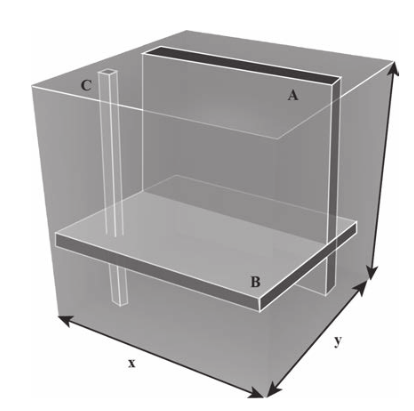
\includegraphics[width=10cm]{datacube.png}
%% \end{figure}

%% \begin{figure}[h]
%%   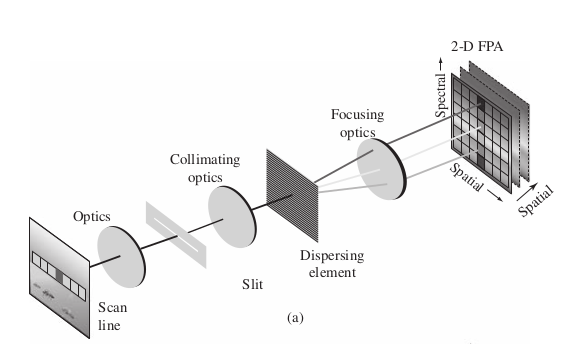
\includegraphics[width=10cm]{pushbroom.png}
%% \end{figure}


%% Different types of rigs:
%% \begin{itemize}
%%   \item Pushbroom scanner (ours)
%%   \item Staring System
%%   \item Fourier Transform Imaging Spectrometer (FTIS)
%% \end{itemize}


%% \subsection{Spatial Sampling}
%% \begin{itemize}
%%   \item ground resolution elements are mapped to picture elements (pixels)
%%   \item IFOV: Instantaneous Field of View
%%   \item Cross track dimension: the projection of the long axis of the slit (i.e. the axis of the pushbroom sensors)
%%   \item Along track dimension: the direction accumulated by traveling
%%   \item Ground Sample Distance: physical size of projected pixel element
%% \end{itemize}


%% \begin{figure}[h]
%%   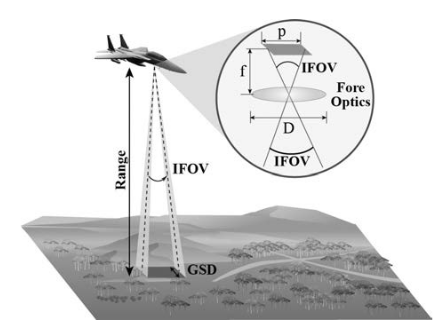
\includegraphics[width=10cm]{scanningProcedure.png}
%% \end{figure}


%% \subsection{Spectral Sampling}
%% \begin{itemize}
%%   \item Recovery of spectral info is imperfect due to finite sampling
%%   \item Spectral Response Function: is the weighing function that describes the wavelengths that are transmitted to a particular spectral sample
%% \end{itemize}

%% \subsection{Radiometric Sampling}
%% \begin{itemize}
%%   \item detector transforms  radiant power to electrical signal
%%   \item electrical signal converted to number via analog-to-digital converter
%%   \item photon detectors
%% \end{itemize}

%% \subsection{Signal Considerations}
%% Strength of signal is determined by:
%% \begin{itemize}
%%   \item Terrain composition affects amount of radiant energy reflected/emitted from ground resolution element
%%   \item Range: Intensity drops off by inverse square law. Further you are away, the worse the signal
%%   \item Spectral Bandwidth: output signal of detector element is proportional to spectral bandwidth of the detector
%%   \item Instantaneous Field of View: Decreasing IFOV increases spatial resolution but weakens the signal
%%   \item Dwell Time: the time required to sweep the IFOV across the ground resolution element, i.e. the time-on-pixel. Longer dwell time $\to$ more accumulated photons $\to$ more signal.
%% \end{itemize}





%% % -------------------------------------------------------------------- %

%% \section{Remote Sensing}

%% mention different types of satellite data platforms (mostly optical), differences in orbits, coverage, etc... Also good to discuss the increasing use of drones for a variety of applications including intelligent agriculture, geophysics, mapping, etc...



%% \subsection{Infrared Sensing Phenomenology}

%% Main passive sources of EM radiation for remote sensing are light emitted by the sun and the self-emission via black-body radiation of objects due to their temperature.

%% \subsection{Sources of Infrared Radiation}
%% \begin{itemize}
%% \item \textbf{spectral radiant exitance} power per unit area emitted by the sun. We can treat this as a black body with temperature $5800 K$, maximum emittance at $\lambda = 0.50$ $\mu m$.
%% \item The Earth is ~$300 K$ with maximum spectral radiant emittance at $\lambda = 9.7$ $\mu m$. This is known as the \textbf{thermal infrared}
%% \end{itemize}

%% \subsection{Atmospheric Propagation}

%% \begin{itemize}
%% \item Key parameter is the \textbf{path length} of atmosphered traveled through before it arrives at the remote sensing system. Main effects are:
%%   \begin{itemize}
%%   \item \textbf{Atmospheric Scattering}: diffusion of radiation by particles in the atmosphere
%%   \item \textbf{Absorption}
%%   \end{itemize}
%% \item Useful remote sensing spectral regions are obtained via the \textbf{Transmission Spectrum}.
%%   \begin{itemize}
%%   \item \textbf{Reflective Range}: $0.35-2.5$ $\mu m$. Dominated by solar illumination
%%   \item \textbf{Water Absorption}: $0.2-2.5$ $\mu m$.
%%   \end{itemize}
%% \item \textbf{Atmospheric Windows}: Regions of low atmospheric absorption
%% \end{itemize}

%% \subsection{Reflectance and Emissivity Spectra}

%% There are three processes that occur when EM radiation meets and interface:
%% \begin{enumerate}
%%   \item \textbf{Reflection}: Solar illumination dominates here. Consequently, this part of the spectrum is used to characterize the surface
%%     \begin{itemize}
%%     \item \textbf{Specular Reflectors}: Flat surfaces that act like mirrors, i.e. $\theta_i = \theta_r$.
%%     \item \textbf{Diffuse (Lambertian) Reflectors}: Rough surfaces that reflect uniformly in all directions.
%%     \item \textbf{Real Reflectors}: Somewhere between the specular and diffuse.
%%    \end{itemize}
%% \item \textbf{Absorption}
%% \item \textbf{Transmission}
%% \end{enumerate}

%% \begin{itemize}
%% \item Fractions vary as a function of $\lambda$
%% \item Remote sensing usually cares about \textit{diffuse} reflectors because this is the dominant type of most materials (water being an exception).
%% \item Reflectance of a material is characterized by its \textbf{Reflectance Spectrum}, that is, the percent of incident light reflected as a function of wavelength.
%%   \begin{itemize}
%%   \item Dips in reflectance spectrum are called \textbf{absorption features}
%%   \item Peaks are called \textbf{Reflectance Peaks}
%%   \end{itemize}
%% \item \textbf{Emissivity Spectrum}: The ratio of radiant emittance at a given temperature to the radiant emittance of a black body at the same temperature.
%% \end{itemize}




% -------------------------------------------------------------------- %

\section{Coordinated Robotic Teams}

we can discuss remote sensing, hyperspectral imaging, and the robot team here... Let's fetch some text from the 2019 paper.

\begin{itemize}
\item Remote Sensing: data acquisition, processing, and interpretation of images, and related data, obtained from aircraft and satellites that record the interaction between matter and electromagnetic radiation
\item Source: the source of electromagnetic radiation, e.g. the sun, black-body radiation, microwave radar, etc...
\item Atmospheric Radiation: The EM radiation propagating through the atmosphere. Moderated by various processes including absorption and scattering
\item Earth's Surface Interactions: Amount and spectral distribution of radiation emitted/reflected by the earth's surface. This depends on
  \begin{itemize}
  \item physical properties of the matter
  \item wavelength of EM radiation that is sensed
  \end{itemize}
\end{itemize}



%% % -------------------------------------------------------------------- %

%% \section{In-situ Chemical Sensing in Water}
%% Here we can give an overview of the sensors utilized on the boat for the robot team studies... We should include any information about the uncertainties. We can also comment on their use in fresh v.s. salt water environments, e.g. we should discuss fluorometers, sonar, and any other relevant sensors from the boat



% -------------------------------------------------------------------- %
\section{A Low Cost Sensor Network For Air Quality Monitoring}
The outdoor part here is optional. Here I seek to provide specific details of the classes of low cost sensors used for PM (optical particle counters based on Mie scattering), thermistors (for tempature), humidity sensors, pressure sensors, gas sensors, etc... This can be a rough outline for those that specifically are used in my research projects.



% -------------------------------------------------------------------- %
\section{PCO and The HEART Chamber}









